%----------------------------------------------------------------------------------------
%	PART: Appendix
%----------------------------------------------------------------------------------------

\part{Appendix}

\chapter{DARC Departments and Required Coursework}\label{Coursework}

Below is a complete listing of the required coursework for each department.


\section{School of Engineering}


\subsection{Intergalactic Astronautics \hfill ING}
\subsubsection{Introduction to Spaceship Design}
Learn spaceship design fundamentals through advanced aeronautics lectures and hands-on projects, including the use of intergalactic CAD to create simulated interstellar vessels.
\subsubsection{Spaceship Engineering I: Materials and Structures}
Delve into advanced spaceship engineering, focusing on materials and structures designed for interstellar travel, supported by hands-on workshops and cutting-edge analysis tools.
\subsubsection{Spaceship Engineering II: Signals and Systems}
Explore the principles of signals and systems in spaceship engineering, covering topics like quantum convolution and hyperfrequency modulation, complemented by lab work in specialized futuristic programming languages.
\subsubsection{Spaceship Engineering III: Fluid Dynamics}
Study fluid dynamics specific to spaceship engineering, investigating phenomena such as shockwave interactions and gravitational flux, with practical labs and projects providing in-depth context.
\subsubsection{Spaceship Engineering IV: Thermodynamics and Propulsion}
Master thermodynamics in spaceship engineering, covering topics from work and heat interactions in a relativistic framework to cosmic propulsion systems, reinforced by hands-on labs.
\subsubsection{Warp Drives and Tenebrivic Propulsion for Astronautics}
Investigate emerging technologies for warp drives and faster-than-light travel, exploring the manipulation of spacetime fabric and dark matter forces, using advanced simulation software for hands-on experience.

\subsection{Xenobiological Engineering \hfill BEX}
\subsubsection{Introduction to Xenobiological Engineering Design Using Synthetic Biology}
Explore synthetic biological systems engineering with a focus on xenobiology, covering topics from DNA synthesis to ethical considerations, preparing students for real-world challenges and interstellar competitions.
\subsubsection{Introduction to Exomachines}
Study the engineering of living exomachines designed for Nyxian use, covering their adaptation and testing, complemented by guest lectures and hands-on projects.
\subsubsection{Advanced Tissue Engineering in Exospecies}
Delve into the principles of tissue engineering for alien species, addressing topics like scaffold design and ethical considerations, while gaining practical lab experience.
\subsubsection{Nanotechnology in Xenobiological Systems}
Examine nanoscale phenomena in Nyxian biology and their applications in human technology, from drug delivery to ethics, through lectures, case studies, and labs.
\subsubsection{Adaptomorphocytic Biology and Interplanetary Epidemiology}
Investigate adaptomorphocytes and their role in interplanetary epidemiology, focusing on their adaptability and impact on diseases, supported by theoretical study and lab research.
\subsubsection{Adaptomorphocytic Static Cells in Carcinogenesis: Origins and Cures}
Explore the role of adaptomorphocytic static cells in cancer progression and treatment, through lectures, literature discussions, and lab exercises focusing on molecular mechanisms and therapeutic interventions.
\subsubsection{Xenofluid Dynamics in Nyxian Physiology}
Learn fluid dynamics in Nyxian biological systems, covering specialized alien organ systems and gaining hands-on lab experience with simulated xenofluidic systems.
\subsubsection{Nyxian Bioauroraescence and Signal Transduction}
Study the biochemical and biophysical mechanisms behind bioauroraescence in alien life, through lectures and labs focused on ion emission, magnetoproteins, and their ecological roles.
\subsubsection{Metagenomics of Nyxian Microbiomes}
Examine Nyxian microbial ecosystems, focusing on their impact on planetary ecosystems and diversity, through hands-on lab sessions and metagenomic data analysis.
\subsubsection{Bioethics in Xenobiological Research}
Address the ethical dimensions of xenobiological research, from biosecurity to intellectual property rights, through case studies, debates, and guest lectures.

\subsection{Tenebrichemical Engineering \hfill BET}
\subsubsection{Fundamentals of Tenebrivity Manipulation}
An introductory course on the engineering of Tenebrivity, the fifth fundamental force linked to dark matter, covering its theory, applications, and potential for sustainable energy, culminating in a hands-on group project.
\subsubsection{Thermodynamics of Tenebrific Systems}
An advanced course on thermodynamics in tenebrific systems, exploring laws, non-equilibrium states, and phase transitions through lectures and lab experiments, focused on sustainable energy applications.
\subsubsection{Material Science in Tenebrific Environments}
Study the material properties influenced by tenebrivity, from metals to nanocomposites, learning techniques for characterization and evaluation, aimed at challenges in tenebrichemical engineering.
\subsubsection{Tenebrichemical Thermodynamics and Propulsion}
Learn engineering principles behind tenebrivity-based propulsion systems for faster-than-light travel, covering efficiency, sustainability, and ethics through experiential labs and team projects.
\subsubsection{Fundamentals of Metabolic and Xenobiochemical Engineering: Applications to Pharmaceutical Xenobiomanufacturing}
Focus on metabolic engineering and xenobiochemical processes in pharmaceutical xenobiomanufacturing, covering topics from cellular optimization to bioreactor design.
\subsubsection{Tenebrific Transport Processes}
Explore heat and mass transfer in tenebrivity-affected systems, emphasizing radiative heat transfer and convective transport, aimed at solving unique engineering problems in this emerging field.
\subsubsection{Nanoscale Tenebrific Energy Transport Processes}
Investigate nanoscale processes affecting energy transport in tenebrific systems, utilizing theories like the Boltzmann transport equation and Marcus electron transfer theory.
\subsubsection{Introduction to Type IV Kardashev Scale Sustainable Energy}
Examine the prospects and challenges of achieving Type IV Kardashev Scale Sustainable Energy, covering a range of energy production techniques and evaluating their engineering, economic, and social impact.
\subsubsection{Fundamentals of Advanced Type IV Kardashev Scale Energy Conversion}
Dive deep into the principles relevant to Type IV Kardashev Scale Energy systems, analyzing efficiency and environmental impact of various energy conversion methods like CO2 capture and fusion power.

\subsection{Superluminal and Interstellar Engineering \hfill LUM}
The Superluminal Engineers are the reason humans can even make it to Nyx and survive the trip without it taking 96 billion years!
\subsubsection{Warp Drive Engineering I: Fundamentals}
Master the basics of warp drive technology for faster-than-light (FTL) travel. Topics include an introduction to spacetime manipulation, exotic matter, and the Alcubierre theory. Engage in labs that prototype miniature warp drive models, with a focus on understanding energy and matter requirements. No prior knowledge of general relativity is required.
\subsubsection{Warp Drive Engineering II: Advanced Theoretical Models}
Dive deeper into the theoretical aspects of warp drive technology. Study advanced spacetime topologies, exotic matter stability, and the latest modifications to the Alcubierre theory. Discuss the feasibility and challenges of warp drive, supported by computer simulations and mathematical proofs.
\subsubsection{Warp Drive Engineering III: Materials and Energy Sources}
Investigate the exotic materials and energy sources required for functional warp drives. Study the physics of negative energy and exotic matter, including their production and stabilization. Hands-on labs focus on material science and high-energy experiments related to warp drive technologies.
\subsubsection{Warp Drive Engineering IV: Capstone Project in FTL Engineering}
Apply your knowledge in a semester-long capstone project, working in teams to design, simulate, and prototype a warp drive system. Topics will range from propulsion and navigation to the ethical implications of FTL travel. Culminates in a peer-reviewed presentation and potential submission for academic journals or intergalactic competitions.
\subsubsection{Introduction to Artificially Conscious Machines}
Explore artificially conscious machines - typically used to manage interstellar travel during human statis - through systems overviews and advanced algorithms. Student projects involve deploying neuro-ethereal sensors and autonomous quantum machines. Background in advanced neural programming recommended.
\subsubsection{Life Support Engineering Design and Superluminal Prototyping}
Design life support systems for high-speed interstellar travel using quantum algorithms and multidimensional matrices. Prototypes are tested in zero-point energy simulations and submitted to an intergalactic competition. Open to all engineering disciplines.
\subsubsection{Operating in the Gaseous Nyxian Environment}
Examine the challenges of operating in the Nyxian environment, blending advanced simulation and lectures from multi-dimensional beings. Teams focus on propulsion and habitat creation for the Intergalactic Nyxian Colonization Program. Limited enrollment, application required.
\subsubsection{Interstellar Traffic Control}
Study traffic control for interstellar routes, exploring astro-navigation and future techniques like tachyonic flux regulation and quantum tunneling. Analyze mission logistics considering time dilation and dark matter. Culminates in a future-focused term paper.


\subsection{Xenophonologic Production \hfill PHO}
\subsubsection{Introductory Articulation Simulation}
Study the Nyxi transarticulator to mimic Nyxi vocal sounds. Learn the nine unique Nyxi consonants through lectures, labs, and computational models. Finish with a project to creattransarticulator.
\subsubsection{Advanced Articulation Simulation}
Advance your knowledge of the Nyxi transarticulator with a focus on mimicking Nyxi triple-pitch vocalizations. Utilize quantum acoustic theories and dynamic simulations to engineer harmonic vocal systems. Features guest lectures from experts.
\subsubsection{Introductory Auroral Production}
Learn the Nyxi's auroral communication, covering syntax, semantics, and auroral symbols. Use simulations and holographic platforms to practice auroral-based phrases. Gain foundational skills for Nyxi auroraphemes.
\subsubsection{Advanced Auroral Production}
Combine Nyxi vocal and auroral communication for enriched meaning. Use neural network simulations and quantum field manipulation for hands-on experience in auroral-sonic patterns. Features Nyxi experts via subspace communication.
\subsubsection{Emissive Engineering}
Understand the engineering of Nyxi auroral emitters. Learn ion production, magnetic field dynamics, and quantum control. Labs focus on building ion emission prototypes. Final project involves designing a basic auroral emitter.
\subsubsection{Nonlinear Emissive Dynamics}
Explore advanced auroral systems mimicking Nyxi patterns. Study nonlinear dynamics like chaos theory and fractal geometry. Use advanced simulations and Nyxi-assisted labs for practical experience.
\subsubsection{Neural Phonotactic Nodes}
Learn to build neural interfaces for direct control of Nyxi phonology and auroral emissions. Covers neural compatibility and machine learning for pattern recognition. Labs include creating neural nodes and interfacing with existing systems.


\subsection{Contraparadoxical Engineering \hfill DOX}
\subsubsection{Fundamentals of Paradox Avoidance}
Learn the basics of paradox prevention within quantum systems, focusing on the principles that guide quantum entanglement, superposition, and wave-function collapse. This course provides an introduction to the key safeguards needed to avoid paradoxical situations like quantum tunneling to prohibited states.
\subsubsection{Temporal Mechanics and Chronostability}
Dive into the intricacies of time travel and explore methods to maintain chronostability. Covering everything from closed timelike curves to branching multiverses, the course equips students to design systems that prevent time loops and chronological inconsistencies.
\subsubsection{Safeguarding Extradimensional Portals and Gateways}
Understand the science of creating and maintaining stable extradimensional portals. Learn to recognize and rectify weak points that could collapse the portal, trapping individuals in pocket dimensions or exposing them to cosmic singularities.
\subsubsection{Holographic Principle and Virtual Reality Paradox Prevention}
Study the intersection of the holographic principle with virtual reality systems. Gain knowledge in ensuring that digital worlds are isolated, preventing the emergence of paradoxical elements like simulated self-aware beings questioning their own existence.
\subsubsection{Recursive System Design and Fractal Safety}
Learn to navigate the risks of engineering systems with recursive elements. This course focuses on avoiding self-referential paradoxes in computational and natural systems, from fractal geometry to recursive algorithms, ensuring they don't reach undefined or catastrophic states.
\subsubsection{Ethical and Social Implications of Contraparadoxical Technologies}
Discuss the ethical boundaries and social implications of deploying technologies that avoid paradoxes. Explore case studies that examine the trade-offs between technological advancements and their potential for unintended, paradoxical consequences on society and reality.


\subsection{Exotic Matter Science and Engineering \hfill MAT}
\subsubsection{Introduction to Exotic Matter}
A foundational course exploring the properties, types, and behaviors of exotic matter, from negative masses to tachyons.
\subsubsection{Warp Drive Engineering for Matter Scientists}
Delve into the principles behind warp drive technologies, focusing on harnessing exotic matter to bend spacetime for faster-than-light travel.
\subsubsection{Wormhole Manipulation}
Learn the theoretical and practical aspects of creating and stabilizing wormholes using exotic matter, with a focus on potential applications.
\subsubsection{Dark Matter and Dark Energy Engineering}
Investigate the properties of dark matter and dark energy, exploring ways to detect, manipulate, and potentially harness them for various applications.
\subsubsection{Exotic Matter in Quantum Computing}
Understand how exotic matter states can influence quantum computation, offering enhanced speed or new paradigms in information processing.
\subsubsection{Casimir Effect and Negative Energy Systems}
Study the Casimir effect in-depth, focusing on the engineering possibilities for negative energy systems and vacuum fluctuations.
\subsubsection{Hawking Radiation and Black Hole Technologies}
Explore the applications of Hawking radiation in the creation of future energy sources, including theoretical black hole power plants.
\subsubsection{Exotic Matter Safety and Ethics}
Examine the ethical considerations and safety protocols essential for research and engineering involving exotic matter forms.


\subsection{Vermiforamenic Medical Engineering \hfill MED}
\subsubsection{Foundations of Vermiforamenology}
Introduction to the principles of vermiforamenology and its integration with medical applications, paving the way for future innovations.
\subsubsection{Wormhole Dynamics in Biomedical Contexts}
Delve into the intricacies of wormhole physics, especially as they relate to biological and medical contexts.
\subsubsection{Nyxian Space-Time Manipulation}
Study the Nyxian techniques for manipulating spacetime and how they can be harnessed for vermiforamenic medical engineering.
\subsubsection{Precision Engineering for Non-invasive Surgery}
Techniques and methodologies for leveraging vermiforamenology for precise, non-invasive surgical interventions.
\subsubsection{Vermiforamenic Imaging Systems}
Explore the engineering of imaging systems that utilize microscopic wormholes for unparalleled clarity and detail.
\subsubsection{Safety and Ethics in Vermiforamenic Engineering}
Discuss the ethical considerations and safety precautions essential when dealing with vermiforamenic technologies.
\subsubsection{Advanced Materials in Wormhole Stability}
Understand the materials science of stabilizing microscopic wormholes and ensuring their safe integration with biological tissues.
\subsubsection{Control Systems for Vermiforamenic Procedures}
Design and optimization of automated systems that control vermiforamenic interventions, ensuring maximum efficacy and safety.
\subsubsection{Integration of AI in Vermiforamenology}
Harnessing artificial intelligence to enhance the predictability, stability, and applications of vermiforamenic practices.
\subsubsection{Vermiforamenic Drug Delivery Mechanisms}
Engineer precise, targeted drug delivery systems using vermiforamenology for optimal therapeutic effects.
\subsubsection{Biocompatibility and Vermiforamenic Interfaces}
A deep dive into ensuring that vermiforamenic systems are biocompatible and do not induce unintended side effects.
\subsubsection{Telemedicine via Vermiforamenic Techniques}
Innovations in providing remote medical care by leveraging vermiforamenic principles for diagnostics and treatment.
\subsubsection{Future Frontiers in Vermiforamenic Engineering}
Engage in speculative and experimental designs in vermiforamenology, charting the next steps in this revolutionary medical field.


\section{School of Expatriation}


\subsection{Enviroadaptive Habitation \hfill HAB}
\subsubsection{Principles of Adaptive Living Systems}
Introduction to the core concepts and technologies that enable habitats to adapt to environmental changes.
\subsubsection{Bio-Responsive Structures}
Study of structures that respond to environmental stimuli using biological principles for optimal sustainability.
\subsubsection{Self-Healing and Regenerative Architecture}
Design and engineering of structures capable of self-repair and regeneration in response to wear and external damage.
\subsubsection{Microclimate Control and Regulation}
Techniques to engineer adaptive microclimates within habitats for enhanced comfort and energy efficiency.
\subsubsection{Symbiotic Urban Planning}
Merging natural ecosystems with urban spaces to create harmonious and adaptive environments.
\subsubsection{Waste-to-Resource Technologies}
Innovations in converting waste products into useful resources within adaptive habitats.

\subsection{Nyxian Architecture \hfill ARC}
\subsubsection{Introduction to Nyxian Spatial Concepts}
Delving into the unique spatial design philosophies of the Nyxi, including their perception of space and function.
\subsubsection{Fluidic and Morphic Design in Nyxian Constructs}
Study of the fluid-like, transformable structures predominant in Nyxian architectural thought.
\subsubsection{Temporal Architectures: A Nyxian Perspective}
Exploration of how Nyxian structures evolve over time and how they interact with their surroundings.
\subsubsection{Acoustics and Resonance in Nyxian Spaces}
Understanding the role of sound and vibration in Nyxian design principles.
\subsubsection{Nyxian Urban Landscapes and Communal Spaces}
A deep dive into the communal and urban spaces of the Nyxi and their integration with natural gaseous elements.


\subsection{Nyxian Social Structures \hfill SOC}
\subsubsection{Nyxian Societal Foundations and Hierarchies}
Overview of the fundamental societal norms, hierarchies, and structures in Nyxian culture.
\subsubsection{Collective Consciousness and the Nyxi}
Exploration of the collective and interconnected consciousness prevalent among the Nyxi.
\subsubsection{Roles and Rituals in Nyxian Society}
Detailed study of the various societal roles and rituals that define Nyxian life.
\subsubsection{Nyxian Art, Expression, and Social Commentary}
Understanding the arts and their role in Nyxian society as mediums of communication and social commentary.
\subsubsection{Interspecies Interactions and Nyxian Diplomacy}
Analysis of how the Nyxi interact with other species and the principles of their diplomatic engagements.


\subsection{Exonutrimental Gastronomy \hfill GAS}
\subsubsection{Introduction to Exonutrimental Cuisine}
Overview of the gastronomic practices that focus on ingredients from Nyxian origins.
\subsubsection{Culinary Techniques for Nyxian Ingredients}
Techniques and methods to prepare, cook, and present foods sourced from beyond Earth.
\subsubsection{Sensory Experiences in Exonutrimental Dishes}
Exploration of the unique sensory experiences associated with consuming Nyxian ingredients.
\subsubsection{Nutritional Science of Nyxian Foods}
Study of the health and nutritional benefits, as well as potential risks, of Nyxian foods.
\subsubsection{Molecular Exogastronomy and Food Chemistry}
Delving into the molecular transformations of Nyxian ingredients in culinary applications.


\subsection{Exoplanetary Geography and Climate Acclimatization \hfill GEO}
\subsubsection{Introduction to Exoplanetary Terrains}
Overview of various types of terrains and landscapes found on exoplanets.
\subsubsection{Exoplanetary Weather Systems and Patterns}
Detailed study of the unique weather systems and patterns present on known exoplanets.
\subsubsection{Human Adaptation to Nyxian Climates}
Exploration of human biological and technological adaptations required for survival in various exoplanetary climates.
\subsubsection{Impact of Nyxian Climates on Infrastructure}
Analysis of the implications of exoplanetary weather on the design and sustainability of infrastructural projects.
\subsubsection{Exoplanetary Hydrology and Oceanography}
Study of liquid systems, including potential oceans, rivers, and lakes, on exoplanets.


\section{School of Nyx Relations}


\subsection{Nyxopology \hfill NYX}
\subsubsection{Introduction to Nyxopology: Landscapes and Features}
Overview of the geographical and geological formations that characterize the Nyxi's home world.
\subsubsection{Flora and Fauna of Nyx}
Study of the unique species and ecosystems endemic to the Nyxi's environment.
\subsubsection{Climatology and Weather Patterns of Nyx}
Detailed analysis of the atmospheric and climatic phenomena of Nyx.
\subsubsection{Subterranean Nyx: Exploring the Underground}
Exploration of the extensive underground networks and environments of the Nyxi's planet.
\subsubsection{Evolving Landscapes: Nyx's Geological History}
A dive into the geological transformations and historic events that have shaped Nyx over eons.


\subsection{Intergalactic Economics \hfill ECO}
\subsubsection{Foundations of Intergalactic Trade}
Core principles and dynamics governing trade between galaxies.
\subsubsection{Currency, Value, and Exchanges in the Cosmos}
Study of the diverse monetary systems and value exchanges prevalent among intergalactic civilizations.
\subsubsection{Intergalactic Supply Chain Dynamics}
Analysis of the complexities involved in the movement of goods across galaxies.
\subsubsection{Economic Policies of Major Cosmic Civilizations}
Exploration of the various economic policies and practices of dominant intergalactic entities.
\subsubsection{The Economics of Stellar Resources}
A deep dive into the value, extraction, and trade of resources found in stars and other cosmic entities.


\subsection{Nyxian History \hfill nxHIS}
\subsubsection{Ancient Nyxi: Origins and Early Civilizations}
A journey into the ancient history, cultures, and civilizations of the Nyxi.
\subsubsection{The Nyxi Renaissance: A Period of Enlightenment}
Exploration of a significant era of Nyxi history marked by cultural, scientific, and artistic flourishing.
\subsubsection{Intergalactic Wars and the Nyxi Role}
Delving into the Nyxi's involvement in major cosmic conflicts and their outcomes.
\subsubsection{Modern Nyxi: Innovations and Evolutions}
A study of recent advancements, societal shifts, and changes within the Nyxi civilization.
\subsubsection{Nyxi Diplomacy: Relations with Other Civilizations}
Examination of the Nyxi's foreign policies, alliances, and interactions with other intergalactic entities.


\subsection{Nyxian Aesthetics and Expression \hfill nxART}
\subsubsection{The Art of the Nyxi: An Overview}
Comprehensive introduction to the myriad forms of artistic expression cherished by the Nyxi.
\subsubsection{Nyxian Music: Soundscapes of Another World}
Exploration of the musical traditions, instruments, and innovations of the Nyxi culture.
\subsubsection{Cosmic Choreography: Nyxian Dance Forms}
Dive into the rhythmic and expressive world of Nyxian dance and performance art.
\subsubsection{Visual Narratives: Nyxian Art and Sculpture}
A journey through the visual arts of the Nyxi, from ancient carvings to modern digital masterpieces.
\subsubsection{Nyxian Fashion and Design}
An exploration of the Nyxi's sense of style, fashion, and design aesthetics.


\subsection{Xenolinguistics \hfill nxLNG}
\subsubsection{Introduction to Xenolinguistics: Beyond Human Languages}
A foundational course offering a broad overview of the field of Xenolinguistics, emphasizing the unique challenges and methodologies associated with studying non-human languages. This course sets the stage for more specialized studies on the Nyxi language.
\subsubsection{Nyxian Phonology: The Art of Nyxian Sound Production}
An in-depth exploration into the nine distinct Nyxi consonant sounds, analyzing their production mechanisms, and highlighting the importance of the Nyxi transarticulator. Through a combination of lectures, practical sessions, and advanced computational modeling, students will gain mastery over the sounds' recreation.
\subsubsection{Nyxian Auroral Semiotics: Deciphering Visual Linguistics}
Dive into the captivating realm of auroral communication as used by the Nyxi, understanding the syntax, semantics, and pragmatics of auroral shapes, colors, motions, and transitions. The course uses immersive simulations and interactive holographic platforms to aid comprehension and production.
\subsubsection{Advanced Nyxian Syntax and Morphology}
Beyond basic structure, this course delves into the intricacies of Nyxian sentence formations, verb conjugations, and the nuances of morphological changes, enabling students to craft complex and meaningful sentences in the Nyxi language.
\subsubsection{Nyxian Lexicology: Building a Nyx-Human Dictionary}
Focusing on the semantics of Nyxi words, this course aims to build a comprehensive lexicon bridging Nyxi and human languages. Through collaborative projects, students will contribute to the ongoing efforts of building a Nyxi-Human dictionary.
\subsubsection{Pragmatics of Nyxian Communication}
Explore the cultural, social, and situational contexts influencing Nyxian language use. This course emphasizes real-world application, analyzing Nyxian language in various contexts, from diplomatic exchanges to artistic performances.
\subsubsection{Neural Linguistic Interfaces in Nyxian Communication}
Study the advancements in neural interfaces that facilitate direct linguistic control over phonology and auroral machinery, understanding the convergence of technology and xenolinguistics in bridging communication gaps.
\subsubsection{Nyxian Poetry and Literature: A Linguistic Analysis}
Dive into the rich literary traditions of the Nyxi, analyzing poetic structures, narrative forms, and linguistic devices. This course offers insights into the Nyxi's cultural and historical contexts through their written and auroral expressions.
\subsubsection{Comparative Studies: Nyxian vs. Earth Languages}
Understand the parallels, contrasts, and unique features of Nyxian language when compared to various Earth languages. Through this comparative approach, students will gain a deeper appreciation of linguistic diversity across civilizations.
\subsubsection{Sociolinguistics of the Nyxi: Language in Society}
Examine the sociocultural factors influencing Nyxian language use, including regional dialects, sociolects, and the implications of language in Nyxian societal hierarchies and identities.
\subsubsection{Nyxian Language Acquisition: Pedagogical Approaches}
Delve into the methodologies and strategies effective for teaching the Nyxi language to humans. This course is especially valuable for those aiming to be educators or linguistic ambassadors in intergalactic exchanges.
\subsubsection{Evolution of Nyxian Language: Historical Linguistics}
Trace the historical evolution of the Nyxi language, identifying ancient forms, understanding linguistic shifts, and predicting future changes in the ever-evolving linguistic landscape of Nyx.
\subsubsection{Digital Tools in Xenolinguistics: Software and Simulations}
Understand the role of advanced software, simulations, and AI in studying and teaching Nyxian language. This course includes hands-on sessions with cutting-edge linguistic software tailored for Nyxian studies.
\subsubsection{Intercultural Communication: Nyxian and Human Dialogues}
Harness the power of effective communication by understanding the cultural nuances, taboos, and etiquette in Nyxian dialogues. Role-playing, simulations, and real-world interactions form core components of this course.
\subsubsection{Nyxian Language and Diplomacy}
Tailored for those with aspirations in intergalactic diplomacy, this course emphasizes the nuanced use of Nyxian language in diplomatic contexts, ensuring precise and effective communication in high-stakes scenarios.


\subsection{Nyxi-Human Relations \hfill nxREL}
\subsubsection{First Contact: The Meeting of Two Civilizations}
In-depth study of the historical event when humans first encountered the Nyxi.
\subsubsection{Diplomacy and Alliances: Navigating Interspecies Politics}
Examination of the political, cultural, and economic ties binding humans and the Nyxi.
\subsubsection{Shared Innovations: Collaborative Projects and Endeavors}
Overview of key collaborative projects undertaken by humans and the Nyxi for mutual advancement.
\subsubsection{Intercultural Exchanges: Learning and Adapting}
Exploration of the rich exchange of ideas, traditions, and knowledge between the two species.
\subsubsection{Challenges and Controversies in Nyxi-Human Relations}
Analysis of the disputes, misunderstandings, and controversies that have arisen and how they were addressed.



\subsection{Extraterrestrial Ethics and Philosophy \hfill nxETH}
\subsubsection{Origins of Nyxian Morality}
A comprehensive study of the ethical foundations of Nyxian civilizations, exploring how environmental factors, evolutionary pressures, and social constructs shape moral codes.
\subsubsection{Comparative Philosophical Systems: Earth vs. Cosmos}
Analyzing philosophical thought across civilizations, this course sheds light on shared universal truths and distinct cosmic perspectives, promoting intergalactic understanding.
\subsubsection{Ethical Dilemmas in Intergalactic Relations}
Delve into real-world cases of ethical challenges faced in interstellar diplomacy, trade, and collaboration, encouraging critical thinking and moral reasoning.
\subsubsection{Metaethics Among the Stars}
Deep dive into the metaethical studies of values, rights, and wrongs as perceived by different cosmic civilizations, exploring relativism, subjectivism, and realism in a vast universe.
\subsubsection{Philosophy of Cosmic Existence}
Explore profound questions of existence, purpose, and reality from the vantage of the vast cosmos, integrating both human and Nyxian viewpoints.


\subsection{Cosmic Extradition and Law \hfill nxLAW}
\subsubsection{Foundations of Cosmic Jurisprudence}
Introduction to the fundamental principles, statutes, and customs that govern the broader cosmic legal systems, setting a basis for advanced legal studies.
\subsubsection{Extradition Treaties Among the Stars}
Study of the intricacies involved in extradition treaties across galaxies, with special focus on Nyxi-human legal relations.
\subsubsection{Rights of Interstellar Beings}
Comprehensive exploration of the rights and protections accorded to sentient beings across the cosmos, emphasizing shared universal rights and species-specific provisions.
\subsubsection{Galactic Trade Laws and Regulations}
Deep dive into the commercial laws that facilitate intergalactic trade, focusing on trade barriers, tariffs, and intellectual property rights in space.
\subsubsection{Dispute Resolution in the Cosmos}
Examination of the mechanisms, institutions, and practices in place to resolve interstellar disputes, from mediation to cosmic courts.


\subsection{Intersentiental Psychology and Behavior \hfill nxPSY}
\subsubsection{Introduction to Intersentiental Cognitive Processes}
Foundational exploration of the cognitive functions and processes of various sentient beings, emphasizing both shared and unique neurobiological mechanisms.
\subsubsection{Emotional Expressions Across the Cosmos}
Study of the myriad ways emotions are expressed, experienced, and perceived among different intergalactic species, with special focus on auroral expressions of the Nyxi.
\subsubsection{Social Behaviors and Group Dynamics in Outer Space}
Delving into the social constructs, hierarchies, and group behaviors of Nyxian civilizations, exploring similarities and differences in social motivations.
\subsubsection{Psychopathologies in the Stars}
A rare look into the mental health challenges faced by various cosmic species, understanding their root causes, manifestations, and potential treatment methodologies.
\subsubsection{Interspecies Relations: Psychology of Interactions}
Exploring the psychological intricacies of interactions between different sentient beings, focusing on biases, misconceptions, and the path towards mutual understanding.



\section{School of Sciences}


\subsection{Physics of Tenebrivity and Aliquantics \hfill TEN}
\subsubsection{Introduction to Tenebrivity}
The basics of dark matter physics, and the foundation of tenebrive forces in the universe.
\subsubsection{Aliquantic Particle Dynamics}
An understanding of the unique, non-standardized particles and their behavior in the quantum realm.
\subsubsection{Tenebrive Waveforms and Interference Patterns}
The study of dark matter-modulated wave properties and the resulting interference in various mediums.
\subsubsection{Aliquantic Fields and Forces}
Exploration of the unique forces exerted by aliquant particles, and how they shape the physical realm.
\subsubsection{Tenebrive Thermodynamics}
Understanding the laws of thermodynamics in environments dominated by dark matter energies.
\subsubsection{Aliquantic Symmetry and Asymmetry}
Exploration of balance and imbalances in aliquant systems.
\subsubsection{Tenebrive Relativity and Inertial Frames}
The relative nature of dark matter-influenced motions and events in spacetime.
\subsubsection{Quantum Tunneling in Aliquant Systems}
The principles of quantum tunneling when influenced by aliquant particles.
\subsubsection{Advanced Tenebrive Optics}
Delve deep into the interaction of dark light and dark matter in controlled and natural settings.
\subsubsection{Unified Aliquantic Field Theories}
Attempts and theories to unify the disparate fields of physics under aliquantic principles.
\subsubsection{Computational Tenebrivity}
Applying computational models and simulations to dark matter-based physics.
\subsubsection{Aliquantic Phenomena in Astronomy}
A study of how aliquantic principles manifest in cosmic and astronomical settings.
\subsubsection{Experiments in Tenebrive Chambers}
Practical laboratory work focusing on controlled dark matter environments.
\subsubsection{Tenebrive Quantum Field Theory}
Bridging the world of quantum mechanics with dark matter-influenced forces and fields.
\subsubsection{Aliquantic Cosmology}
The study of the universe's origin, evolution, and eventual fate through the lens of aliquant physics.


\subsection{Xenobiology and Nebugenomics \hfill BIO}
\subsubsection{Intro to Xenobiological Taxonomy}
Classification and categorization of Nyxian life forms based on morphological and genetic traits.
\subsubsection{Principles of Nebugenomics}
Understanding the genetic blueprints of non-Earth organisms and their interpretation.
\subsubsection{Xeno-ecosystems and Habitats}
Study of alien ecological systems and the dynamics between various xenobiological species.
\subsubsection{Nebugenic Mutation and Evolution}
Exploration of the mutation rates, causes, and their influence on Nyxian species evolution.
\subsubsection{Xenobiological Physiology}
The study of the physical and chemical functions of Nyxian organisms.
\subsubsection{Advanced Nebugenic Techniques}
Laboratory techniques specific to the study and manipulation of alien genes.
\subsubsection{Extraterrestrial Ethology}
Behavior study of alien species in their natural environments.
\subsubsection{Nebugenic Diseases and Immunity}
Study of diseases in alien species and their unique immune responses.
\subsubsection{Xenobiological Reproduction and Life Cycles}
Delve into the reproductive mechanisms and stages of life in Nyxian species.
\subsubsection{Nebugenomics and Technological Applications}
Exploring the applications of alien genetics in biotechnology.
\subsubsection{Exobiological Conservation and Ethics}
Conservation methods and the ethical considerations in xenobiological research.
\subsubsection{Nebugenic Data Analysis and Bioinformatics}
Utilizing computational tools to analyze vast genetic datasets from alien species.
\subsubsection{Comparative Planetology and Life Potential}
Comparison of different planetary environments and their potential to harbor life.
\subsubsection{Nebugenic Engineering and Synthetic Biology}
The principles and techniques to engineer and modify alien genetic codes.
\subsubsection{Interstellar Biogeography}
Study of the distribution of life forms across star systems and potential patterns.


\subsection{Tenebrichemistry and Quantavistics \hfill CHM}
\subsubsection{Introductory Tenebrichemistry}
Foundations of dark matter-influenced chemical reactions and understanding matter transformations under tenebrive influences.
\subsubsection{Quantavistic Dynamics}
Deep dive into the motion and interaction of quantavistic particles and their implications in modern chemistry.
\subsubsection{Tenebrous Molecular Structures}
Study of molecular formations in tenebrive environments, focusing on stability, bonding patterns, and reactivity.
\subsubsection{Quantavistic Thermodynamics}
Thermodynamic principles as applied to the realm of quantavistics.
\subsubsection{Applied Tenebrichemical Engineering}
Practical applications of tenebrichemistry in novel materials and medicines.
\subsubsection{Quantavistic Kinetics}
Understanding reaction rates and mechanisms in the domain of quantavistic chemistry.
\subsubsection{Interplay of Light and Shadows in Tenebrichemistry}
Delve into how photonic interactions influence chemical reactions in tenebrive settings.
\subsubsection{Nano-scale Tenebrichemistry}
Exploration of dark matter chemistry at atomic and molecular scales.
\subsubsection{Tenebrive Catalysis}
Understanding how tenebrive influences can act as catalysts in chemical reactions.
\subsubsection{Advanced Quantavistic Simulations}
Hands-on approach to model and simulate quantavistic reactions using modern computational tools.
\subsubsection{Emerging Materials in Tenebrichemistry}
Study of novel materials emerging from dark matter-influenced chemical reactions.
\subsubsection{Quantavistic Reaction Mechanisms}
Deep understanding of how quantavistic particles interact and transform during chemical reactions.
\subsubsection{Tenebrichemical Energy Systems}
Exploration of energy storage and release in tenebrive chemical systems.
\subsubsection{Safety in Tenebrichemistry Labs}
Best practices and protocols to handle tenebrive chemicals and processes safely.
\subsubsection{Tenebrichemistry in Biology}
Understanding the influence and implications of tenebrive chemical processes in living organisms.


\subsection{Exoneuroscience and Polyphrenic Consciousness \hfill CON}
\subsubsection{Basics of Exoneural Structures}
Introduction to the neural configurations of Nyxian beings.
\subsubsection{Polyphrenic Cognitive Processes}
Study of non-terrestrial thought processes, emotions, and memories. Gain a deep understanding of Nyxian cognition, which relies on a polyphrenic consciousness
\subsubsection{Exoneural Signal Transduction}
Study of unique signaling pathways in Nyxian nervous systems.
\subsubsection{Consciousness Across Cosmos}
Comparative study of consciousness across different species.
\subsubsection{Nyxian Sensory and Perception Systems}
Exploration of the sensory organs of non-Earth life forms.
\subsubsection{Neuroplasticity in Exoneural Systems}
Analysis of adaptability and flexibility in alien neural networks.
\subsubsection{Psychoactive Substances in Nyxian Species}
Examination of natural and artificial substances that affect consciousness in Nyxian beings.
\subsubsection{Evolution of Exoneural Systems}
Study of the evolutionary pathways and factors influencing exoneural development.
\subsubsection{Polyphrenic Dream Analysis}
Dive into the world of dreams and subconscious processes in the Nyxians who have multiple consciousnesses.
\subsubsection{Comparative Study of Neural Pathways}
Contrast and comparison of neural pathways across species from various planets.
\subsubsection{Exoneurochemical Interactions}
Understanding neurotransmitter systems and chemistry in alien neural structures.
\subsubsection{Cognitive Augmentation in Nyxian Species}
Exploration of natural and technological means of enhancing cognition in Nyxian beings.
\subsubsection{Neuroethical Considerations in Exoneuroscience}
Delving into the ethical implications of studying and interacting with alien neural systems.
\subsubsection{Neural Basis of Nyxian Emotions}
Deep dive into the neural underpinnings of emotions in Nyxian species.
\subsubsection{Interspecies Neural Communication}
Exploration of possible communication avenues between human and alien neural systems.


\subsection{Galactostructural and Exoplanetary Sciences \hfill GAL}
\subsubsection{Exoplanetary Geology and Tectonics}
Understanding geophysical properties and tectonic activities on exoplanets.
\subsubsection{Galactic Structures and Morphologies}
Study of diverse architectures and forms of galaxies.
\subsubsection{Exoplanetary Atmospheres and Climates}
Study of the atmospheric compositions and climates of planets beyond our solar system.
\subsubsection{Galactic Nucleosynthesis and Star Evolution}
Exploration of element formation in galaxies and the life cycles of stars.
\subsubsection{Advanced Exoplanetary Geophysics}
Dive into core, mantle, and crust interactions on alien planets.
\subsubsection{Exoplanetary Oceans and Hydrospheres}
Study of water and liquid formations on planets, understanding their influence on habitability.
\subsubsection{Galactic Black Holes and Singularities}
In-depth exploration of the most enigmatic structures in galaxies.
\subsubsection{Astrobiology and Signs of Life}
Search and study of life or its signs in various planetary environments.
\subsubsection{Exoplanetary Magnetospheres and Radiation Belts}
Understanding the magnetic fields of planets and their implications for life.
\subsubsection{Galactic Collisions and Mergers}
Exploration of the dynamics and outcomes of galaxies merging and interacting.
\subsubsection{Exoplanetary Volcanology}
Study of volcanic activities and their implications on alien planets.
\subsubsection{Stellar Lifecycles in Diverse Galaxies}
Deep dive into how stars form, evolve, and end in different galactic environments.
\subsubsection{Interstellar Medium and Cosmic Dust}
Exploration of the material that exists in the space between the stars in a galaxy.
\subsubsection{Gravitational Waves and Cosmic Disturbances}
Study of ripples in spacetime caused by some of the most violent and energetic processes in the cosmos.
\subsubsection{Exoplanetary Habitability and Terraforming}
Exploring the criteria for planetary habitability and the prospects and ethics of terraforming.


\subsection{Novomathics \hfill MTH}
\subsubsection{Fundamentals of Nyxian Numerals}
Exploration of the Nyxian numerical system, its base, and its historical development. Students will learn the symbolic representations, conversion techniques, and basic arithmetic operations.
\subsubsection{Geometry in Higher-Dimensional Spaces}
Dive into the study of shapes, sizes, properties, and dimensions of things in higher-dimensional Nyxian spaces. This course covers the basic to advanced properties of hyper-shapes and their practical applications.
\subsubsection{Nyxian Algorithms and Computation}
An introduction to the logic and algorithms specific to Nyxian mathematics. This course emphasizes computational efficiency, error handling, and Nyxian-specific problems.
\subsubsection{Quantum Probabilistics}
A comprehensive study of probability in the context of quantum mechanics, allowing students to model and predict Nyxian quantum phenomena with newfound precision.
\subsubsection{Fractal Dynamics and Nyxian Patterns}
Understand the recursive nature of fractals in Nyxian mathematics, exploring both their theoretical foundations and practical applications in various fields like architecture, art, and natural phenomena.
\subsubsection{Temporal Mathematics and Paradox Resolution}
Dive into the mathematical models used to describe and resolve temporal anomalies. This course covers the mathematical techniques to predict and counteract paradoxical scenarios in time-based experiments.
\subsubsection{Nyxian Cryptomathematics}
Study the art and science of encoding and decoding information in the Nyxian way. This course sheds light on historical and modern cryptographic techniques, emphasizing Nyxian unique mathematical principles.
\subsubsection{Tensor Calculus in Curved Spacetime}
Delve into advanced mathematical techniques used to describe phenomena in curved spacetime environments, such as gravitational fields around massive celestial bodies or the warping effects near wormholes.
\subsubsection{Nyxian Topology and Continuity}
An exploration of the properties of space that are preserved under continuous deformations. This course will delve into the Nyxian understanding of closeness, limits, and continuous transformations.
\subsubsection{Abstract Algebra and Nyxian Structures}
A deep dive into the algebraic structures of the Nyxian mathematical system, focusing on groups, rings, fields, and their respective applications in various Nyxian technologies.
\subsubsection{Mathematical Logic and Nyxian Propositions}
Examine the foundational principles of logic from a Nyxian perspective, from basic propositional logic to advanced topics in predicate logic and set theory.
\subsubsection{Computational Complexity in Exotic Systems}
Understand the limitations and capabilities of Nyxian computational devices. Explore the P-NP problem, computational hierarchies, and the challenges of solving problems in alien systems.
\subsubsection{Nyxian Game Theory and Strategic Interactions}
Study the mathematical models of strategic interaction among rational Nyxian entities, encompassing evolutionary games, coalition formations, and multi-agent systems.
\subsubsection{Differential Equations in Dynamic Systems}
Tackle the mathematical descriptions of how things change and evolve in the Nyxian universe, from simple linear equations to complex, nonlinear dynamics.
\subsubsection{Set Theory and Infinite Nyxian Constructs}
Venture into the world of infinite sets, cardinalities, and ordinal numbers, all within the framework of Nyxian mathematical traditions. Understand the hierarchy of infinities and their implications in Nyxian cosmology.


\chapter{Xenochemistry}

\section{The Periodica Tenebris}\label{PeriodicaTenebris}

The Periodica Tenebris is the Periodic Table of Dark Matter, only developed after collaboration with the Nyxi.
\\
\begin{center}
  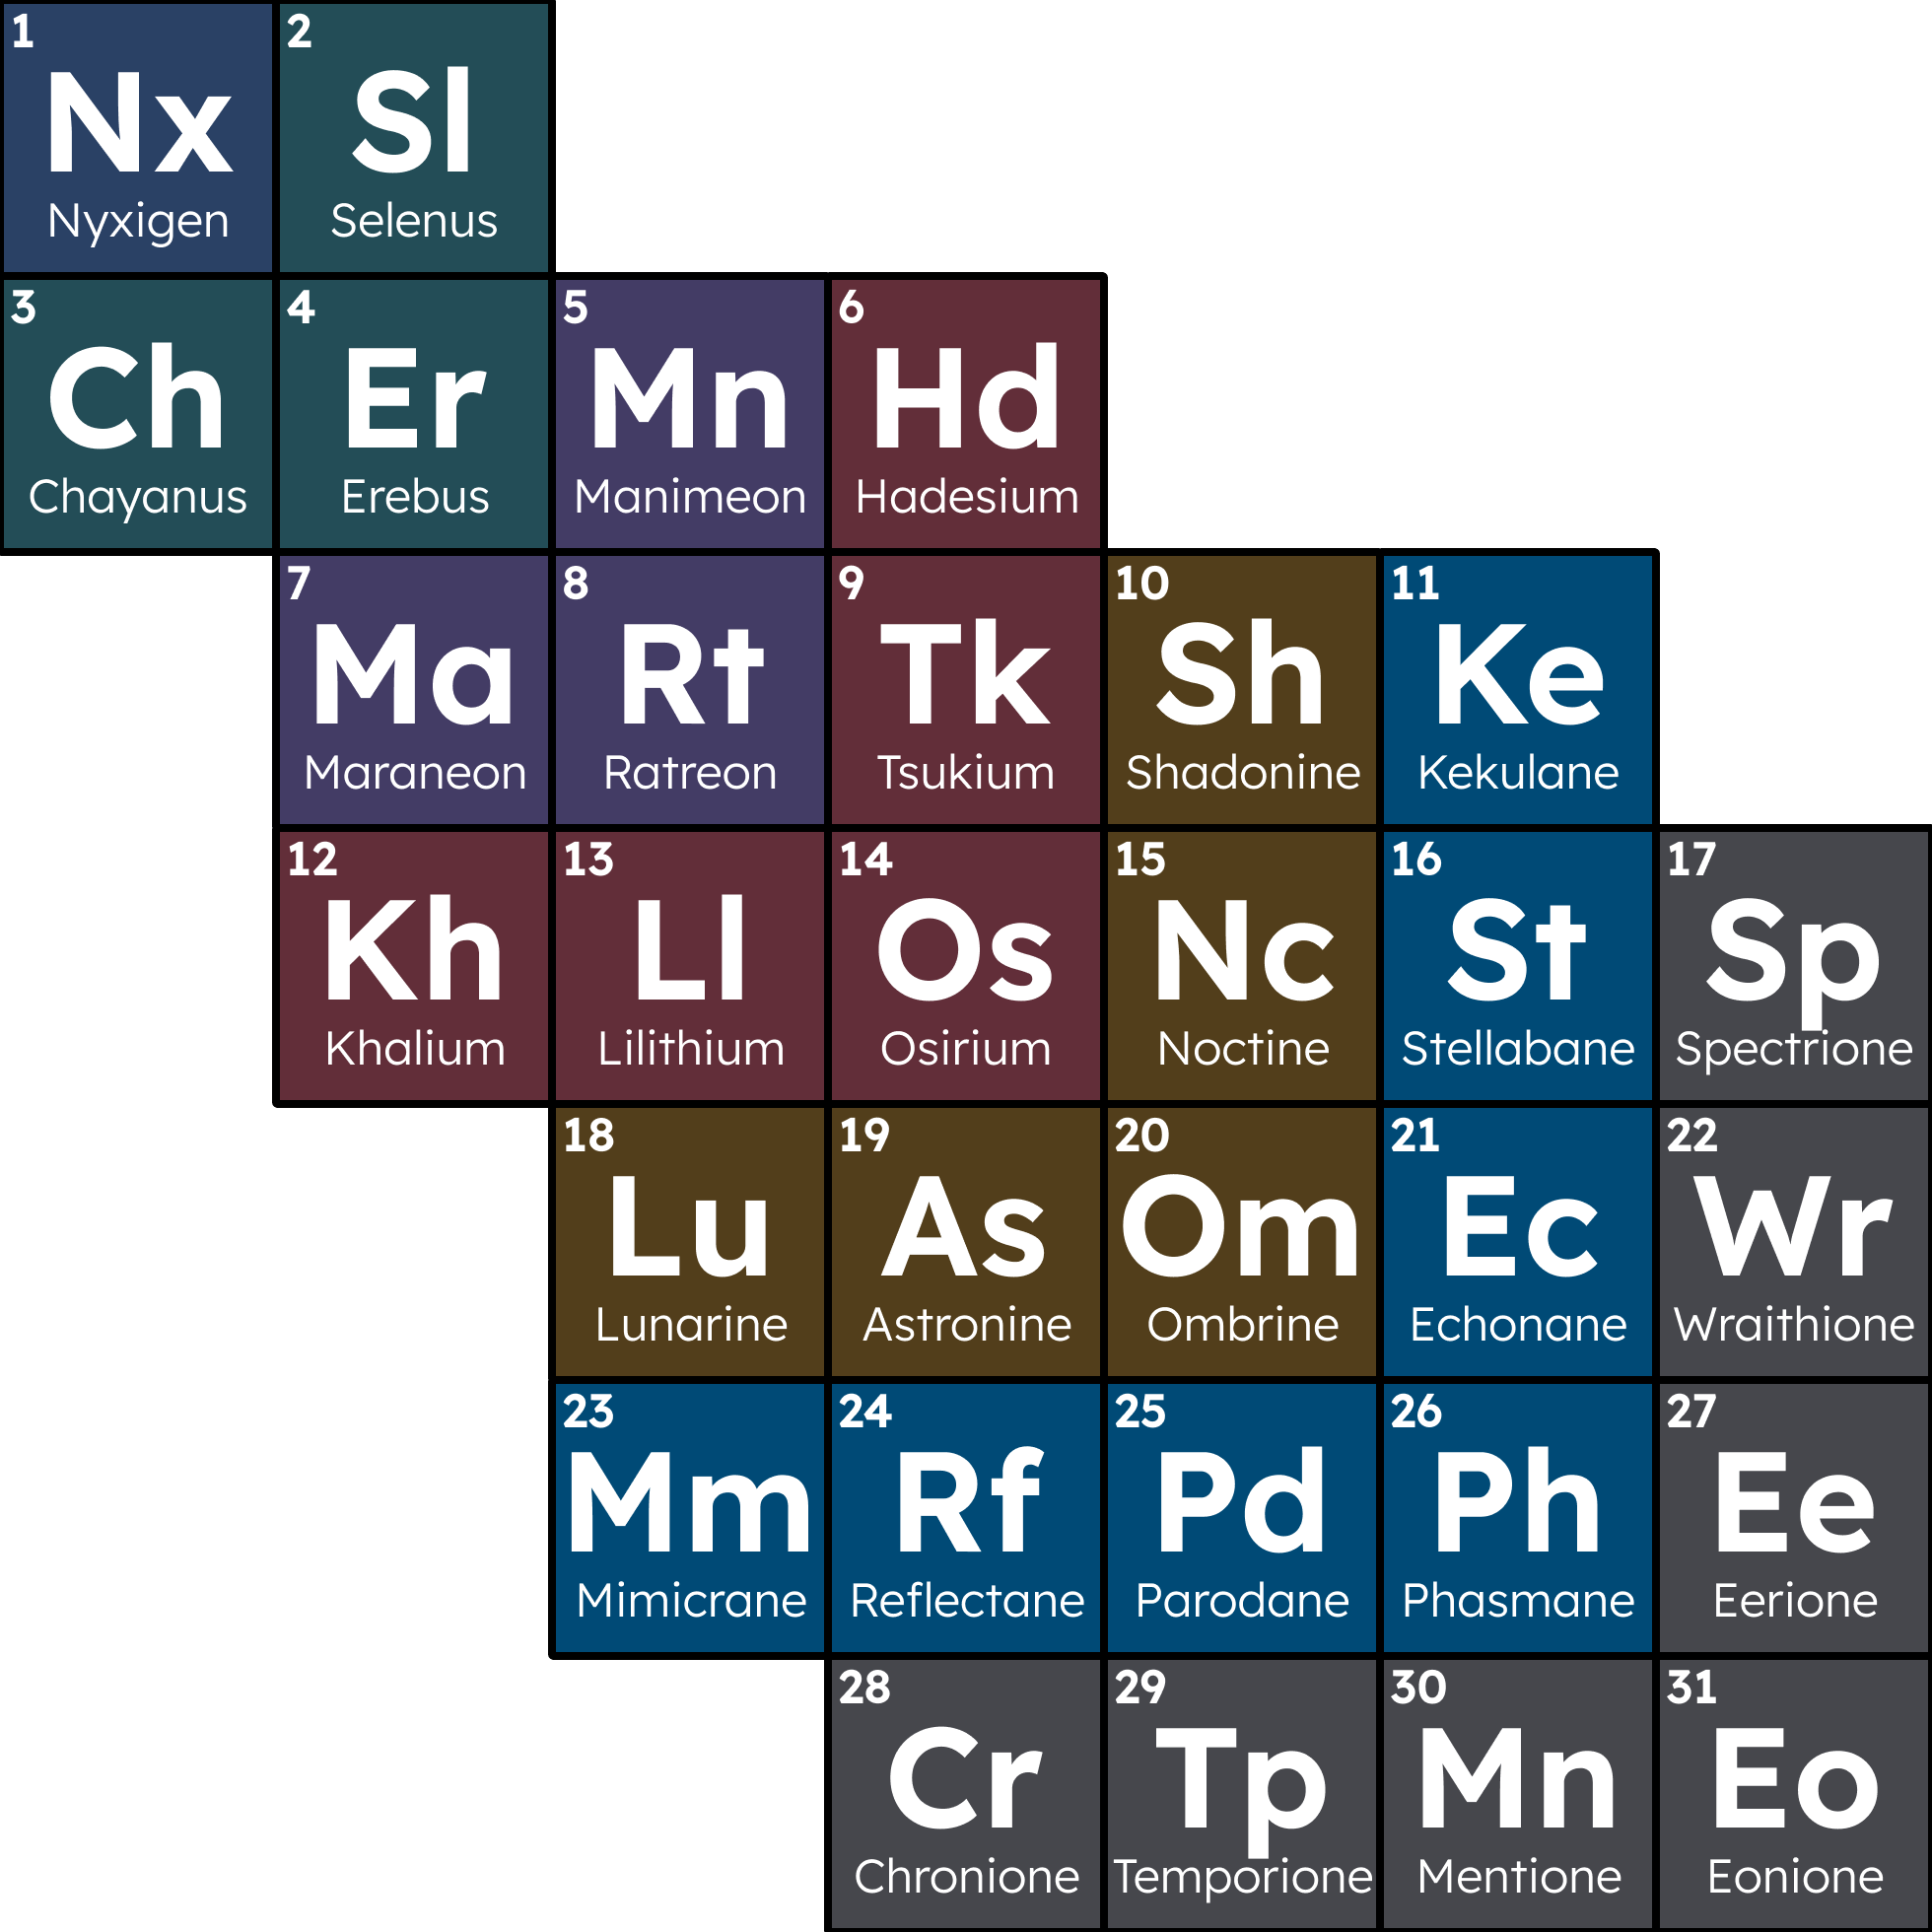
\includegraphics[width=0.7\textwidth]{Periodica_Tenebris.png}
\end{center}

%----------------------------------------------------------------------------------------
%	BIBLIOGRAPHY
%----------------------------------------------------------------------------------------

\chapter*{Bibliography}
\addcontentsline{toc}{chapter}{\textcolor{ocre}{Bibliography}}
\section*{Books}
\addcontentsline{toc}{section}{Books}
\printbibliography[heading=bibempty,type=book]
\section*{Articles}
\addcontentsline{toc}{section}{Articles}
\printbibliography[heading=bibempty,type=article]

%----------------------------------------------------------------------------------------
%	INDEX
%----------------------------------------------------------------------------------------


\cleardoublepage
\phantomsection
\setlength{\columnsep}{0.75cm}
\addcontentsline{toc}{chapter}{\textcolor{ocre}{Index}}
\printindex

%----------------------------------------------------------------------------------------